\subsection{Signal Start Detection}
\label{subsec:03_signalStartDetection}

As mentioned in \cref{sec:02_signalStartDetection}, the detection of the
signal start is crucial for the localization.
Tests showed that the accuracy of the whistle detection is not
sufficient to be used stand alone concerning the start index.
Thus, different approaches are evaluated with regard to higher
precision and lower computational effort.

The implementation of the different approaches will be presented coupled with
an examination of real measurement data.
To reduce undesirable effects and demonstrate the simplest form, a sinusoidal
signal of $3\si{\kilo\hertz}$ was recorded with the same circumstances as the
whistle-sounds.
For the following data, the sound source was placed $2\si{m}$ in front of the robot.
In order to find the time point where the signal starts, information about
smaller fractions are required.
So, the original $44100$ samples that were buffered by the
\lstinline!WhistleLocalization! module are divided into several overlapping
frames with size $256$. The computational effort rises with smaller frame size,
but delivers a higher precision in return.
In order to perform the \ac{FFT} most efficiently, the size of one frame
should be a power of 2.
To compute the entropy, the frames are transformed into
frequency domain with the \ac{FFT}.
The \ac{ZCR} does not require such a transformation.
For the reason that the start detection through analyzing the energy requires a fixed
threshold which varies depending on the environment strongly, it will not be covered
with regard to the signal start detection.
In the evaluation \cref{sec:04_signalStartDetection}, the result of the single
methods are compared to each other.
For better visualization, the following data is shortened to $2400$ samples.

\subsubsection*{Spectral Entropy}

The formula to calculate the spectral entropy of a signal is introduced as
\cref{eq:02_entropy} in the previous chapter.
For the entropy information, the signal should not be cleaned previously.
The point at which the signal changes from noise to whistle-signal was found by
computing the finite differences between the sampling points of the entropy.
This approach is not real-time capable but introduces a small delay.
\Cref{fig:03_entropy} is a plot of the recorded sine signal with the corresponding
entropy.
According to the frame size, the accuracy of the start index can be increased.
However, the frame size is limited by the required number of samples for one \ac{FFT} and
its computational effort.
In \cref{subsec:04_entropy}, the entropy outcome of a whistle-sound
and its derivation is presented for evaluation.
% -------------------------------------------------------------
\begin{figure}[ht]
	\centering
		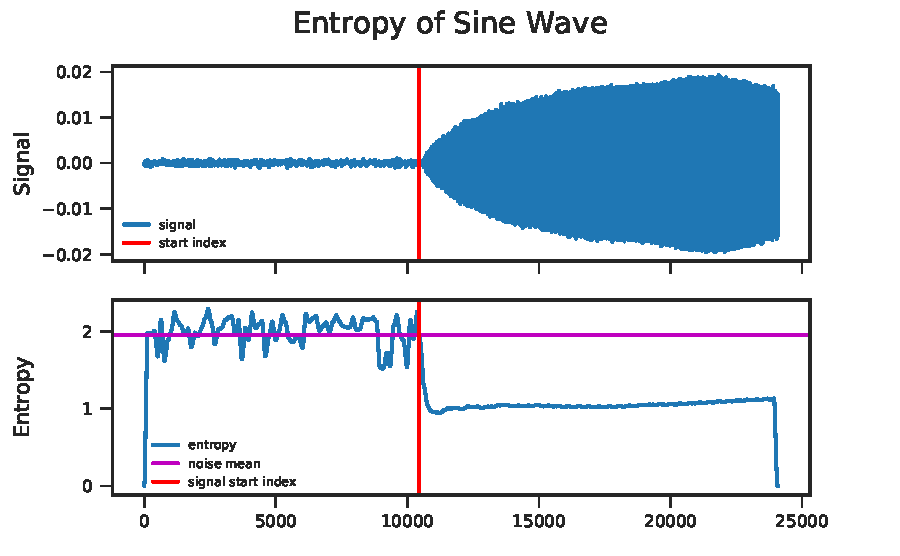
\includegraphics[]{figures/sine_entropy}
	\caption{Exemplary entropy of a sinusoidal signal with 3\si{\kilo\hertz}.}
	\label{fig:03_entropy}
\end{figure}
% -------------------------------------------------------------

% \subsubsection*{Energy}

% \info[]{need to be written up}
% As mentioned above, the total signal is divided into multiple overlapping frames.
% \Cref{eq:02_spectralEnergy} represents the energy of each frequency
% component.
% According to this, the energy of one of those frames is \cref{eq:02_energy}.
% Assuming that the energy holds for the entire frame, overlapping and adding the energy
% results in \cref{fig:03_energy}.
% If the frequency of the examined signal is known as for the whistle, only energy values
% of the relevant frequencies need to be considered.
% One downside of the energy information is that the threshold has to be adapted
% manually for the related environment.
% Especially for competitive tournament conditions with varying and unforeseeable noise levels,
% parameters like these should be avoided and thus,
% the start detection by energy is inconvenient.
% % -------------------------------------------------------------
% \begin{figure}[ht]
% 	\centering
% 		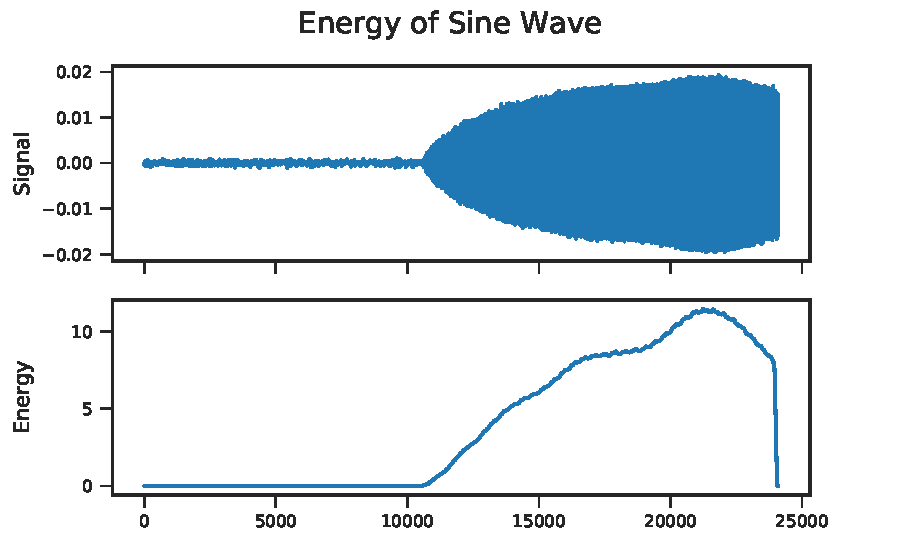
\includegraphics[]{figures/sine_energy}
% 	\caption{Energy of a sinusoidal signal with 3\si{\kilo\hertz}.}
% 	\label{fig:03_energy}
% \end{figure}
% % -------------------------------------------------------------

\subsubsection*{Zero Crossing Rate}

Alike the other methods, the buffered signal is divided into smaller frames
which can be set arbitrarily small for the \ac{ZCR} where no \ac{FFT} is necessary.
% To receive a higher accuracy, the frames of the \ac{ZCR} can be set small.
% are set to 80 samples.
In each frame, the sign changes are counted which only requires simple implementation
and is computationally lightweight.
An assumption in this work is that the signal is represented at the
end of the received data and that only noise exists at the beginning.
Using this condition, the \ac{ZCR} of the first few frames is averaged and
defined as noise \ac{ZCR} mean value.
On the other hand, the same can be done with frames at the end of the data to
provide a signal \ac{ZCR} mean.
By comparing both means, a dynamic threshold can be defined which can be
adjusted depending on the circumstances optionally.
Better results could be obtained by reversing the signal and
determining the index where the signal fell below the threshold.
Number of noise and signal frames are parameter values which depend
on the amount of samples and the size of the frame.
% In \cref{fig:03_zcr} and in this work, the threshold is set by multiplying the
% mean of the noise and signal mean by factor 1.25.
\begin{figure}[ht]
	\centering
		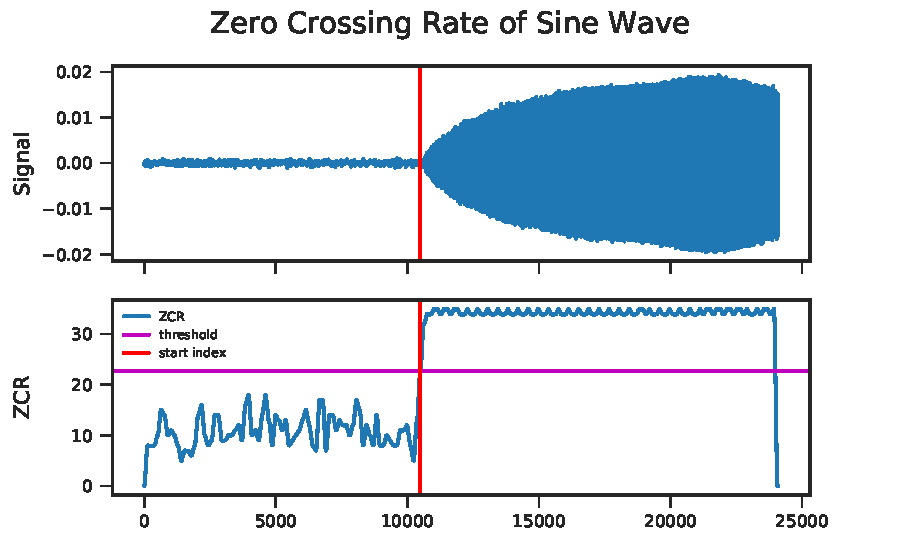
\includegraphics[]{figures/sine_zcr}
	\caption{Zero Crossing Rate of a sinusoidal signal with 3\si{\kilo\hertz}.}
	\label{fig:03_zcr}
\end{figure}
